% ===========================================================================
% Section 10. Designing the Allied Industrial Base: a network optimization
% Specification: R/indices/allied_network_design.R and scripts/30_build_allied_network_design.R.
% Numbers: final full rerun of 2026-10-12, scripts/30 at lambda = 0.78 (paper/results/network.json,
% network_frontier.json). Algorithms, EU-node rules and the lambda grid: Appendix C
% (app:algorithm). Further results: Online Appendix oa:network (sections/oa_network.tex).
% Robustness of the design (fig:network_robustness, tab:network_robustness): Section 11.
% ===========================================================================
\section{Designing the Allied Industrial Base: a network optimization}
\label{sec:network}

The indices of Sections~\ref{sec:es}--\ref{sec:bilateral} score countries, sectors and pairs one at
a time. The case for an Allied Industrial Base turns on a different question
\citep{neis2026allied}: a top-ranked country may add little if its strengths duplicate the
coalition's, and a lower-ranked one may complete a resilient chain, so the object is a country's
marginal contribution to the system and the task is to optimise combinations rather than rankings.
The same source sketches a portfolio objective, security, opportunity, development and durability
gains net of cost premia, delay, duplication and residual coercion exposure, maximised under
explicit constraints such as a resilience floor and minimum diversity; because the weights are
political, it asks for a frontier of feasible choices rather than one correct weighting.

This section builds the part of that objective that the indices support. For each Upstream and
Midstream stage of the eleven headline technologies, a mixed-integer program chooses which network
nodes produce, what share each carries and which partners each supplies. It rewards fit, the
capability of producers and the quality of their partnerships, and penalises concentration through
a concave Herfindahl term, under share limits, a dual-sourcing floor and caps on the number of
stages a node may lead; the penalty weight traces a frontier between fit and dispersion, and a rule
picks one point on it. The program is a multi-sourcing variant of facility-location and network
design \citep{geoffrion1974multicommodity,owen1998strategic,melo2009facility,daskin2013network}
with dual-sourcing constraints \citep{tomlin2006value,snyder2016orms}. Its objective is a score, not
a cost, and the design is normative: it describes what a planner with these preferences would
choose, not where production will locate. Appendix~\ref{app:algorithm} states the algorithms and
Online Appendix~\ref{oa:network} reports further results.

% ---------------------------------------------------------------------------
\subsection{Nodes, stages and scores}
\label{subsec:network_sets}

The network consists of the 57 coalition members of Section~\ref{sec:coalition} (31 core members
and 26 partners) and the six EU members that belong to it only through the Union. The EU-27 is one
node, so the 63 economies form 37 nodes; its inputs are aggregated from the members with the stage
weights of Section~\ref{sec:coalition}, and edges between members are internal and dropped
(Appendix~\ref{app:algorithm}). Taiwan, Switzerland and the China-leaning suppliers outside the
coalition are not nodes. A stage is a technology with $s\in\{\text{Upstream},\text{Midstream}\}$,
22 in all; Downstream deployment serves each member's own market and is not part of the allied
division of labour. All 37 nodes enter every stage, each as a potential producer $p$ and as a
consumer $c$.

Within each stage, $\EO$ and $\ES$ are re-ranked across the nodes with the S-curve of
Section~\ref{sec:normalization}, $\tilde v_p=\Scurve(r_p)$ with $r_p=(\rank(v_p)-1)/(n_v-1)$ and
$\gamma=0.5$, so that a score measures a node's standing among its partners. The producer score is
the weighted mean of the components observed,
\begin{equation}\label{eq:net_producer_score}
  a_p=\frac{\sum_{v\in\{\EO,\ES\}}\omega_v\,\1[\tilde v_p\ \text{observed}]\,\tilde v_p}
           {\sum_{v\in\{\EO,\ES\}}\omega_v\,\1[\tilde v_p\ \text{observed}]},\qquad
  (\omega_{\EO},\,\omega_{\ES})=(0.5,\,0.2),
\end{equation}
that is, $5/7$ and $2/7$ when both are observed. Opportunity is the index closest to productive
capability; security enters as reliability, since a secure node is a steadier supplier. The Policy
index is not part of the score: its basis differs across members (IEA PAMS alone for 11 of them),
and it enters the allied picks of Section~\ref{sec:strategic} instead. In the two Geothermal stages
no node has $\ES$; in Green Hydrogen Midstream five small partners lack it.

Demand is an allocation key, not a forecast. With need $1-\widetilde{\ES}_c$ and size the S-curve of
the rank of GDP \citep{worldbank2026wdi},
\begin{equation}\label{eq:net_demand}
  \tilde d_c=
  \begin{cases}
    \tfrac12\,(1-\widetilde{\ES}_c)+\tfrac12\,\mathrm{size}_c & \text{if } \widetilde{\ES}_c \text{ is observed},\\
    \mathrm{size}_c & \text{otherwise},
  \end{cases}
  \qquad d_c=\tilde d_c\Big/\textstyle\sum_{c'}\tilde d_{c'} .
\end{equation}
Because both terms are S-curved ranks, demand is rank-compressed: the EU node, with 24.6\% of the
nodes' GDP, has a median weight of 0.035 across stages, close to the United States' 0.033, and no
node has more than 0.054 in any stage. Development potential (Section~\ref{sec:bilateral}) has zero
weight in the objective and serves only to rank build candidates (Online
Appendix~\ref{oa:network}).

% ---------------------------------------------------------------------------
\subsection{Partnership edges}
\label{subsec:network_edges}

The quality of supply from $p$ to $c$ combines the two directed partner indices of
Section~\ref{sec:bilateral}, each read from the end it describes: the consumer's friendshore rating
of the producer and the producer's opportunity rating of the consumer's market,
\begin{equation}\label{eq:net_edge}
  W_{pc}=\tfrac12\,\FS_{cpts}+\tfrac12\,\PO_{pcts},\qquad p\neq c .
\end{equation}
Friendshore carries the consumer's view of the producer as a friendshoring opportunity, where the
consumer's security need meets the producer's economic opportunity on existing trade and investment
ties, including UN-vote alignment and Chinese ownership of the producer's foreign-invested
manufacturing. A missing component counts as zero. Of the 29{,}304 stage-specific ordered pairs of distinct nodes, 90.3\% carry both
components and 9.7\% friendshore only (every pair in the two Geothermal stages and the 180 pairs
with a Green Hydrogen Midstream consumer without $\ES$); none has neither. Self-supply is valued at
the median edge of the stage,
\begin{equation}\label{eq:net_self_edge}
  W_{pp}=\operatorname{median}\{W_{qc}:\ q\neq c,\ W_{qc}\ \text{observed}\},
\end{equation}
so domestic supply competes with a typical partnership, with neither home bias nor penalty.

% ---------------------------------------------------------------------------
\subsection{The stage program}
\label{subsec:network_program}

For stage $(t,s)$ the decisions are the flows $f_{pc}\ge0$, the share of the coalition's unit
demand that $p$ supplies to $c$; the selection indicators $y_p\in\{0,1\}$; and the link indicators
$\ell_{pc}\in\{0,1\}$. Production shares are $x_p=\sum_cf_{pc}$, and the program is
\begin{subequations}\label{eq:net_milp}
\begin{align}
  \max_{f,\,y,\,\ell}\quad
    & J=\sum_{p,c} f_{pc}\,\big(w_N\,a_p+w_E\,W_{pc}\big)+w_D\sum_p\delta_p\,y_p-\lambda\sum_p x_p^2
    \label{eq:net_obj}\\
  \text{s.t.}\quad
    & \textstyle\sum_p f_{pc}=d_c && \forall c, \label{eq:net_c_demand}\\
    & \underline s\,y_p\le x_p\le\bar s\,y_p,\qquad \textstyle\sum_p y_p\ge m_P && \forall p, \label{eq:net_c_share}\\
    & \varepsilon\,d_c\,\ell_{pc}\le f_{pc}\le d_c\,\ell_{pc},\qquad \ell_{pc}\le y_p,\qquad
      \textstyle\sum_p\ell_{pc}\ge m_S && \forall p,c, \label{eq:net_c_link}\\
    & y_p=0 && \forall p\in\mathcal{X}_{ts}, \label{eq:net_c_elig}
\end{align}
\end{subequations}
with $w_N=1$, $w_E=0.5$, $w_D=0$, $\bar s=0.40$, $\underline s=0.05$, $m_P=3$, $m_S=2$,
$\varepsilon=0.10$ and $\lambda=0.78$, where $\mathcal{X}_{ts}$ holds the nodes barred by the
portfolio caps. Demand is met in full by network producers (the network is closed); no node carries
more than 40\% of a stage and a selected one at least 5\%, a stand-in for minimum efficient scale;
and every consumer has at least two suppliers, each carrying at least a tenth of its demand. These
constraints bound the Herfindahl index of designed shares, $\HHI^{\mathrm{D}}_{ts}=\sum_px_p^2$
\citep{hirschman1945national}, for any $\lambda$:
\begin{equation}\label{eq:net_hhi_bounds}
  \frac{1}{\min\{|\mathcal{E}_{ts}|,\lfloor 1/\underline s\rfloor\}}
  \ \le\ \HHI^{\mathrm{D}}_{ts}\ \le\
  \lfloor 1/\bar s\rfloor\,\bar s^{2}+\big(1-\lfloor 1/\bar s\rfloor\,\bar s\big)^{2}=0.36,
\end{equation}
where $\mathcal{E}_{ts}$ is the set of eligible producers.

The term $-\lambda\,\HHI^{\mathrm{D}}_{ts}$ is the diversification penalty, in score units per unit
of concentration. Without it the objective is linear and the solution sits at corners, two
producers at the cap and a third with the remainder. With it the marginal value of a share falls
with its size, and at an interior optimum two producers' shares differ by their difference in
marginal value divided by $2\lambda$: at $\lambda=0.78$ a score advantage of 0.0156 buys one
percentage point of share. The penalty plays the role of the variance term in portfolio choice
\citep{markowitz1952portfolio}, without a model of disruption probabilities, and it is the part of
the program that values a node by what it adds to a combination: once the leaders' marginal value
has fallen, a lower-scoring node with good partnerships enters. If supplier outages were
independent and equally likely, with probability $\pi$, the variance of the share of a stage lost
would be $\pi(1-\pi)\HHI^{\mathrm{D}}_{ts}$, so $\lambda$ reads as a price of that variance. The
penalty is additively separable, however: a producer's marginal penalty depends only on its own share,
and every node counts as an independent source, so two producers that share a bloc, a region or a
Chinese parent diversify as much as two unrelated ones. The design is therefore a first step toward
optimising combinations, not its full form (Section~\ref{sec:discussion}). The MILP carries the penalty
through tangent cuts on a share grid of 0.01, in perspective form (error at most
$2.5\times10^{-5}$ per producer; Appendix~\ref{app:algorithm}). Stages are built with
\texttt{ompr} \citep{schumacher2023ompr} and solved by GLPK \citep{makhorin2020glpk} under a
300-second limit, with a greedy water-filling heuristic as fallback.

% ---------------------------------------------------------------------------
\subsection{Portfolio caps}
\label{subsec:network_portfolio}

Solved independently, the stages would select the same strong nodes again and again,
concentrating the base in a few economies and leaving many members without a stake. The design
therefore caps the number of stages in which a node is a leading producer, rising with the
logarithm of GDP:
\begin{equation}\label{eq:net_cap}
  \kappa_i=\min\Big\{\kappa_{\max},\,\max\Big\{\kappa_{\min},\
  \operatorname{round}\Big(\kappa_{\min}+(\kappa_{\max}-\kappa_{\min})\,
  \frac{\eta_i-\min_{j}\eta_j}{\max_{j}\eta_j-\min_{j}\eta_j}\Big)\Big\}\Big\},
\end{equation}
where $\eta_i=\log(1+\mathrm{GDP}_i)$, $\kappa_{\min}=2$, $\kappa_{\max}=10$ for the largest economy, and the EU's GDP summed over its
members. A node's appearances are the stages in which it is among the five largest producers,
\begin{equation}\label{eq:net_topk}
  A_i=\big|\big\{(t,s):\ x_{i,ts}>0,\ \rho_{i,ts}\le K\big\}\big|,\qquad K=5,
\end{equation}
where $\rho_{i,ts}$ is a strict rank of the share (ties broken by producer score, then by code), so
a stage contributes at most five appearances. After all stages are solved, each node with
$A_i>\kappa_i$ is barred from the $A_i-\kappa_i$ stages in which its share times its score is
smallest, those stages are re-solved, and the count is repeated until no node exceeds its cap: a
heuristic coupling of the stages, not a joint optimum.

% ---------------------------------------------------------------------------
\subsection{Calibrating the diversification weight}
\label{subsec:network_calibration}

No price converts concentration into score, so $\lambda$ is set by a rule with an observable
anchor: the smallest value on a grid at which the median of $\HHI^{\mathrm{D}}_{ts}$ over the 22
stages is at most the median export Herfindahl index of the nodes themselves,
$\HHI^{\mathrm{N}}_{ts}$, over the 18 stages with an HS6 basket (all but Geothermal and Green
Hydrogen). $\HHI^{\mathrm{N}}_{ts}$ uses 2024 basket exports from the reconciled all-reporter
Comtrade matrix \citep{uncomtrade}, with shares within the 37 nodes and the EU counting only its
extra-EU exports. The target is 0.1556 (6.43 equivalent exporters). The design should be no more
concentrated, in the median stage, than the coalition's own exports already are; a closed network
of 37 nodes cannot match the dispersion of a world market, so world concentration would be the
wrong anchor.

The grid has 36 points (0, 0.5, every 0.01 from 0.70 to 1.00, and 1.1, 1.2 and 1.5), each a full
re-solve of the production configuration. The rule picks $\lambda=0.78$, at which the median is
0.1520, or 6.58 effective producers (Figure~\ref{fig:network_frontier}; Appendix~\ref{app:algorithm}
tabulates the grid). The pick is knife-edge. At 0.77 the median is 0.1558, missing the target by
0.0002; the median is not monotone in $\lambda$ (it rises in eight of the 35 grid steps, from
0.1485 at 0.79 to 0.1502 at 0.80, for instance), because interior shares move top-five membership
and the portfolio loop then bars different nodes; and the pick moved with every revision of the
inputs during the final data corrections. The rule, not the number, is therefore the specification,
re-applied to every full rerun. The design it selects is less fragile than the number: at
$\lambda=0.77$ and 0.79 at most 1.1\% of production moves in the mean stage
(Section~\ref{sec:robustness}). The frontier prices diversification in score, not in resource costs: at the pick the summed node
and edge terms are 5.8\% below their value at $\lambda=0$, at $\lambda=1.5$ (median index 0.095)
10.6\% below. This is the frontier of choices the conceptual objective asks for
\citep{neis2026allied}.

\begin{figure}[htbp]
  \centering
  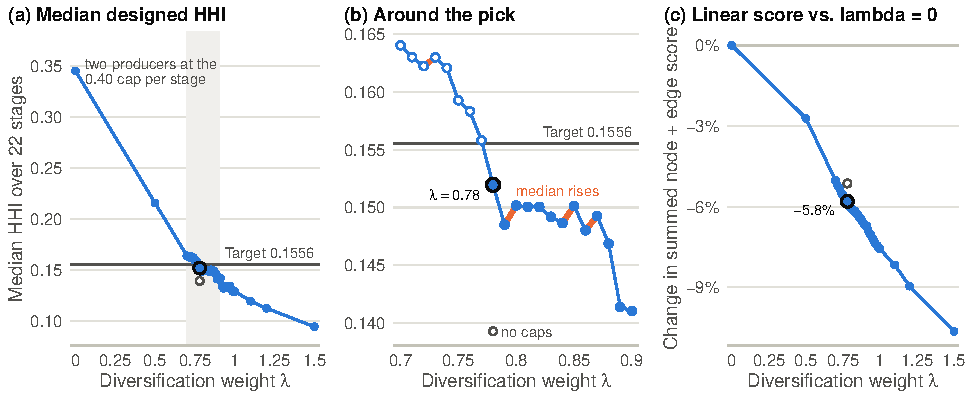
\includegraphics[width=\textwidth]{network_frontier}
  \caption{Calibration of the diversification weight $\lambda$. Panel~(a): median over the 22
  Upstream and Midstream stages of the Herfindahl index of designed production shares at each of
  the 36 grid values of $\lambda$ (37 nodes, portfolio caps on, MILP with a 300-second stage
  limit); the horizontal line is the target, the median export Herfindahl index of the nodes over
  the 18 basket stages (0.1556); the large marker is the pick, $\lambda=0.78$; the open circle the
  same design without portfolio caps. Panel~(b): the neighbourhood $0.70\le\lambda\le0.90$; open
  markers lie above the target, filled markers meet it, and orange segments are steps at which the
  median rises although $\lambda$ increases. Panel~(c): the summed node and edge terms of the 22
  stage objectives, without the Herfindahl penalty, in percent of their value at $\lambda=0$.
  Source: calibration study on the inputs of the final rerun of 12 October 2026.}
  \label{fig:network_frontier}
\end{figure}

% ---------------------------------------------------------------------------
\subsection{Results}
\label{subsec:network_results}

\paragraph{Solution.} All 22 stages are solved by the MILP, none by the fallback, and the
portfolio loop converges after seven passes; the 62 stage solves take 462 seconds, none more than
10.6.

\paragraph{Who produces what.} Figure~\ref{fig:network_specialization} and
Table~\ref{tab:network_producers} show the designed division of labour: 201 producer roles, from
seven producers (Nuclear Upstream) to ten per stage, median nine. $\HHI^{\mathrm{D}}_{ts}$ runs from
0.126 (Oil Midstream) to 0.209 (Nuclear Upstream); the largest share is 0.325 (Indonesia in Green
Hydrogen Upstream, Canada in Nuclear Upstream), none reaches the cap, and 61 sit at the floor. Twenty-nine of the 37
nodes produce somewhere; eight never do (Turkey, New Zealand, Ukraine, the Dominican Republic,
Guatemala, Ghana, Costa Rica and Gabon). Canada has the most roles (16), then the EU node (15; it leads no stage), the United States and
Indonesia (13 each). How many roles a node takes follows its size through the caps
(Spearman correlation 0.75 with the cap); which stages it takes follows its scores. Nodes outside
the high-income group carry 47\% of designed Upstream and 43\% of Midstream production.

Three patterns arise from the construction rather than from observed capacity. Indonesia,
China-leaning by its votes and a member through IPEF, leads six Upstream stages and Oil Midstream:
the producer score has no alignment term, which reaches the design only through the edges.
Thailand leads both Geothermal stages, where scores rest on $\EO$ alone and edges lack their
opportunity half. And the design applies no endowment screen: by the screen of the allied picks
(Section~\ref{sec:strategic}), 21 of the 90 designed roles in the ten screened Upstream stages are
held by nodes without recorded reserves or production of the stage's resources, a median of 11\% of
stage production (none in Electric Vehicles, Gas and Oil Upstream; 36\% in Solar Upstream). Their
shares are supply they would have to source through trade or overseas equity.

% Generated by scripts/paper/fig_network.R from data/processed/outputs/allied_network_specialization.csv
\begin{table}[htbp]
\centering
\begin{threeparttable}
\caption{Designed producers and production shares by technology and stage}
\label{tab:network_producers}
\footnotesize
\begin{tabularx}{\textwidth}{@{}>{\raggedright\arraybackslash}p{2.1cm} >{\raggedright\arraybackslash}X >{\raggedright\arraybackslash}X@{}}
\toprule
Technology & Upstream & Midstream \\
\midrule
Batteries & IDN~.23, AUS~.22, CAN~.12, CHL~.12, ARG~.08, PHL~.06, EU~.06, GBR~.05, ZAF~.05 & USA~.29, IND~.14, MYS~.14, CAN~.11, EU~.10, THA~.06, KOR~.06, GBR~.05, JPN~.05 \\
Coal & IDN~.26, IND~.15, VNM~.12, COL~.09, ZAF~.07, PER~.07, CAN~.06, THA~.06, EU~.05, PHL~.05 & JPN~.20, EU~.20, COL~.14, KOR~.12, VNM~.08, CAN~.07, ISR~.06, MEX~.05, MYS~.05 \\
Electric Grid & CHL~.31, MEX~.14, COD~.12, PER~.12, PHL~.07, AUS~.05, GBR~.05, JPN~.05, NOR~.05, ZAF~.05 & THA~.22, MEX~.15, JPN~.13, MYS~.11, EU~.10, USA~.08, CAN~.05, IDN~.05, IND~.05, MAR~.05 \\
Electric Vehicles & IDN~.24, AUS~.21, USA~.16, CHL~.08, PHL~.07, ARG~.06, EU~.05, THA~.05, ZAF~.05 & USA~.32, MEX~.20, KOR~.19, JPN~.08, VNM~.06, CAN~.05, GBR~.05, ZAF~.05 \\
Gas & USA~.25, CAN~.14, NOR~.14, QAT~.12, MYS~.10, IDN~.05, AUS~.05, IND~.05, OMN~.05, SAU~.05 & IND~.24, USA~.18, EU~.14, KOR~.12, MEX~.06, GBR~.05, IDN~.05, ISR~.05, JPN~.05, NOR~.05 \\
Geothermal & THA~.26, MYS~.15, NOR~.13, ISR~.10, EU~.08, IDN~.07, MEX~.05, CAN~.05, QAT~.05, USA~.05 & THA~.26, MYS~.15, ISR~.14, NOR~.10, QAT~.07, EU~.07, CAN~.06, IDN~.05, MEX~.05, USA~.05 \\
Green Hydrogen & IDN~.33, THA~.14, CAN~.14, EU~.12, MEX~.09, ISR~.08, GBR~.05, PHL~.05 & USA~.26, EU~.21, VNM~.14, NOR~.08, PHL~.07, SGP~.07, KOR~.06, ISR~.05, JPN~.05 \\
Nuclear & CAN~.33, NAM~.22, IND~.16, ZAF~.14, ISR~.05, SAU~.05, THA~.05 & IND~.24, EU~.20, JPN~.14, MYS~.12, ISR~.07, KOR~.06, NOR~.06, GBR~.05, MEX~.05 \\
Oil & USA~.23, SAU~.17, CAN~.17, NOR~.12, OMN~.08, QAT~.08, IDN~.05, IND~.05, THA~.05 & IDN~.20, IND~.14, KOR~.14, THA~.13, VNM~.09, JPN~.08, EU~.06, CAN~.05, MYS~.05, NOR~.05 \\
Solar & IDN~.24, CAN~.15, EU~.12, GBR~.12, NOR~.10, ZAF~.10, IND~.07, SGP~.06, MEX~.05 & IND~.28, USA~.20, VNM~.14, THA~.12, PHL~.06, CAN~.05, JPN~.05, KOR~.05, SGP~.05 \\
Wind & IDN~.22, USA~.22, AUS~.20, JPN~.08, ZAF~.06, CAN~.06, ISR~.05, KOR~.05, SGP~.05 & IND~.28, USA~.25, EU~.15, JPN~.09, MEX~.06, BRA~.06, KOR~.05, VNM~.05 \\
\bottomrule
\end{tabularx}
\begin{tablenotes}[flushleft]\footnotesize
\item \emph{Notes:} Producers of each stage in the production design (37 network nodes, diversification weight $\lambda=0.78$, portfolio caps on, every stage solved by the MILP), ordered by the designed production share $x_{p,ts}$, the share of the coalition's unit demand in the stage that the node supplies (ISO3 codes; EU = the EU-27 node; shares sum to one within a cell and are printed to two decimals). Source: \texttt{allied\_network\_specialization.csv}.
\end{tablenotes}
\end{threeparttable}
\end{table}


\begin{figure}[htbp]
  \centering
  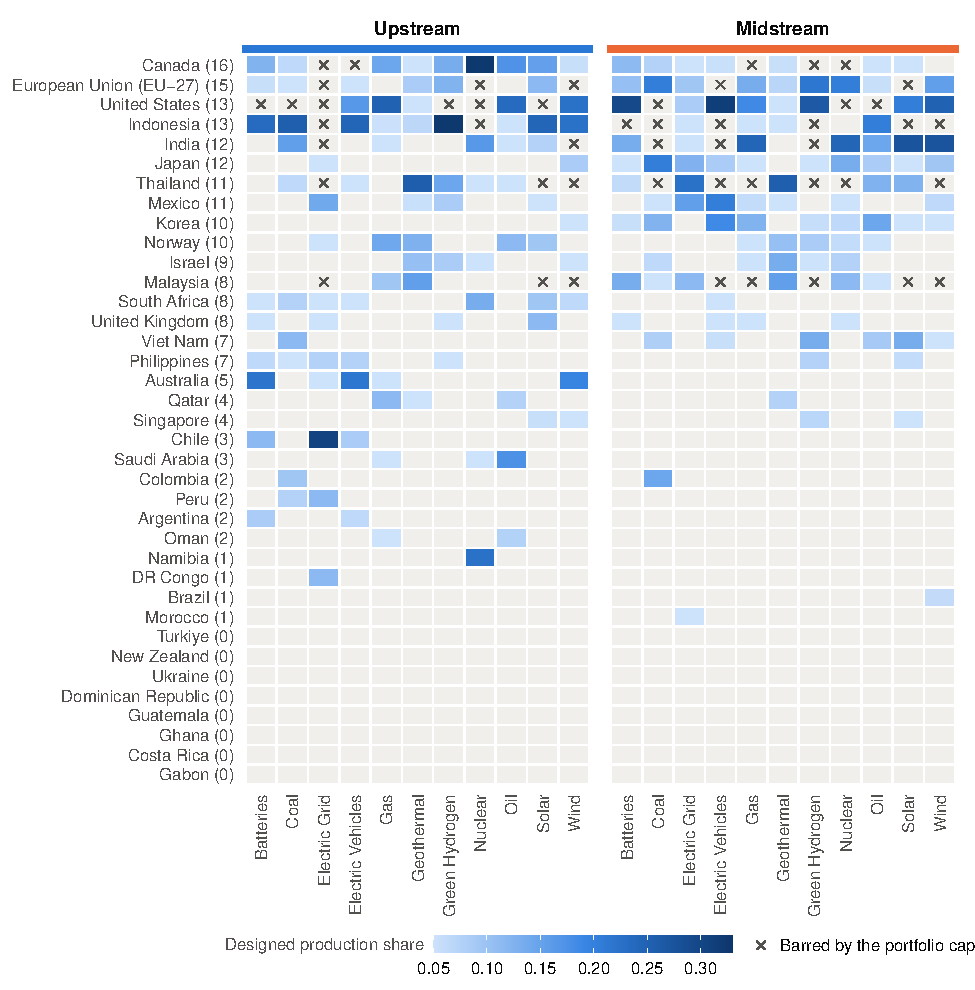
\includegraphics[width=\textwidth]{network_specialization}
  \caption{Designed division of labour across the allied network. Rows are the 37 network nodes
  (the EU-27 as one node), ordered by the number of stages in which they produce (in parentheses)
  and then by their summed share; columns are the eleven headline technologies within the
  Upstream and Midstream stages. Shading is the designed production share $x_{p,ts}$ from the
  floor 0.05 to the largest share, 0.325; light grey cells are stages in which the node does not
  produce, and a cross marks a stage from which the portfolio loop barred the node in its final
  pass. Production design: $\lambda=0.78$, GDP-log portfolio caps, node policy term off, all 22
  stages solved by the MILP. Source: \texttt{allied\_network\_specialization.csv} and
  \texttt{allied\_network\_diagnostics.csv}.}
  \label{fig:network_specialization}
\end{figure}

\paragraph{Flows.} Figure~\ref{fig:network_map} shows three Midstream stages; India leads Solar and
Wind Midstream (0.275 each) and the United States Batteries Midstream (0.295). The redundancy rules
bind: 793 of the 811 consumer--stage pairs with positive demand draw on exactly two suppliers, and
in every stage the weakest link carries exactly 10\% of its consumer's demand. With no transport cost in the objective, routing follows the edge weights: the flow-weighted edge weight is
0.874 in the median stage against an unweighted mean of 0.58, and 15 to 28\% of the mapped flows
stay within a World Bank region.

\begin{figure}[htbp]
  \centering
  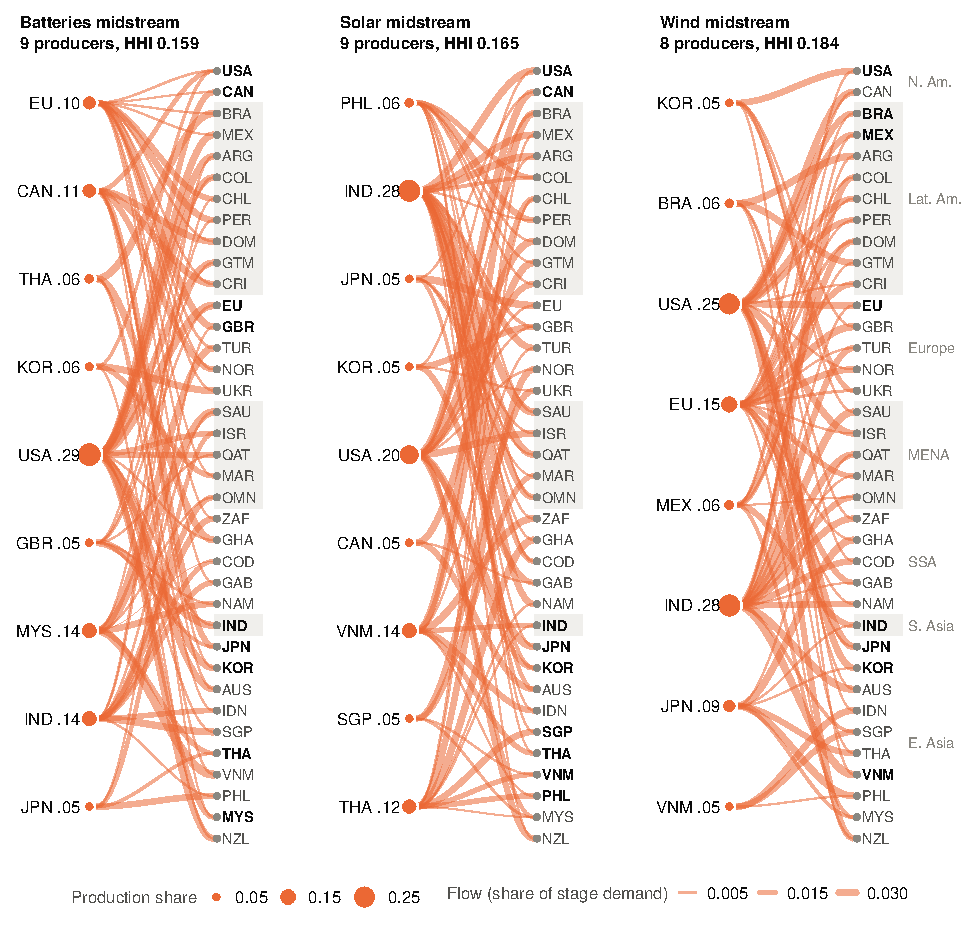
\includegraphics[width=\textwidth]{network_map}
  \caption{Designed flows in three Midstream stages. In each panel producers sit on the left,
  sized by their production share (printed next to the code; EU = the EU-27 node), and all 37
  nodes sit on the right as consumers, in the same order in every panel: by World Bank region
  (shaded bands) and by GDP within region. A line is a flow $f_{pc}$, wider for larger flows;
  consumers that also produce are in bold. Producers are placed at the flow-weighted mean position
  of their consumers (the barycentre step of a two-layer layout computed with \texttt{igraph}
  \citep{csardi2006igraph}). Panel titles give the number of producers and
  $\HHI^{\mathrm{D}}_{ts}$. Production design ($\lambda=0.78$, portfolio caps, MILP). Source:
  \texttt{allied\_network\_flows.csv} and \texttt{allied\_network\_specialization.csv}.}
  \label{fig:network_map}
\end{figure}

\paragraph{Concentration and current exporters.} Figure~\ref{fig:network_concentration} sets the
design against two benchmarks in the 18 basket stages. It meets the nodes' median export
concentration by construction, but stage by stage the two are unrelated (Spearman correlation
$-0.07$): the design spreads production where the nodes' exports are concentrated, as in Nuclear
Upstream (Canada 54\% of node exports), and concentrates it where they are dispersed. It is less
concentrated than world exports (median 0.101) in only five stages. What changes is the identity of
suppliers: China is the largest world exporter in ten basket stages (20 to 43\% of world exports),
and the 37 nodes hold 74\% of world exports in the median basket stage, so the closed design
replaces by assumption 3 to 46\% of current world supply, at a cost the model does not measure. Nor does it follow the ranking of current exporters: in the
median basket stage 66\% of designed production lies outside the three largest exporting nodes, and
designed and observed export shares have a median Spearman correlation of 0.53. Economies that do
not report to Comtrade enter these benchmarks only through their partners' mirror declarations.

\begin{figure}[htbp]
  \centering
  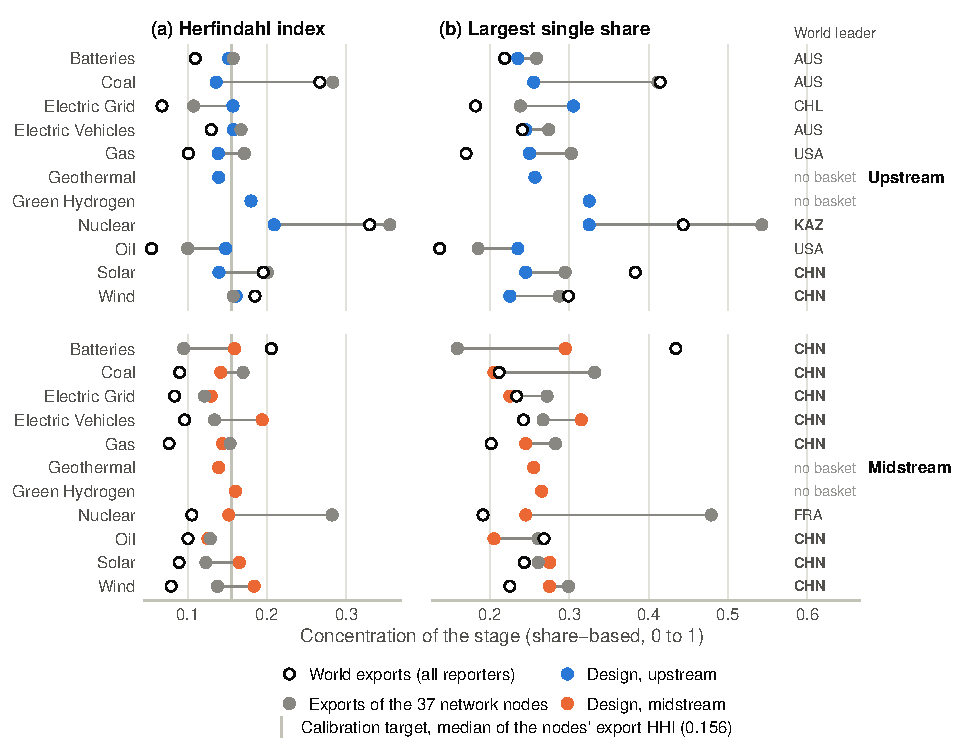
\includegraphics[width=\textwidth]{network_concentration}
  \caption{Designed versus observed concentration by technology and stage. Panel~(a): Herfindahl
  index of designed production shares, $\HHI^{\mathrm{D}}_{ts}$ (filled circles coloured by
  stage); of the 2024 basket exports of the 37 nodes, $\HHI^{\mathrm{N}}_{ts}$ (grey; the EU-27 as
  one exporter counting only extra-EU exports; reconciled Comtrade matrix, importer report else the
  exporter's mirror $\times1.06$); and of world exports across all reporters,
  $\HHI^{\mathrm{W}}_{ts}$ (open circles). The vertical line is the calibration target (0.156).
  Panel~(b): the largest single share in each case; the codes at the right name the world's
  largest exporter of the stage's basket, in bold where it is outside the network. Geothermal and
  Green Hydrogen have no basket. Production design ($\lambda=0.78$, caps on). Sources:
  \texttt{allied\_network\_diagnostics.csv}, \texttt{allied\_network\_observed\_hhi.csv}, UN
  Comtrade \citep{uncomtrade}.}
  \label{fig:network_concentration}
\end{figure}

\paragraph{Portfolio caps.} The caps range from two (Gabon, Namibia) to ten (the United States, the
EU) and sum to 218, against 110 top-five appearances; eight nodes end at their cap, and the final
pass bars 49 (node, stage) combinations in 17 stages (Figure~\ref{fig:network_portfolio}). Without
caps, the United States would be a top-five producer in 17 stages against a cap of ten. The caps
pass appearances chiefly to Japan, Mexico, the Philippines, South Africa and Israel, cost 1.9\% of
the summed objective (at most 5.9\%, in Coal Midstream) and raise the median $\HHI^{\mathrm{D}}_{ts}$
from 0.139 to 0.152, so the calibrated $\lambda$ is specific to the capped configuration.

\begin{figure}[htbp]
  \centering
  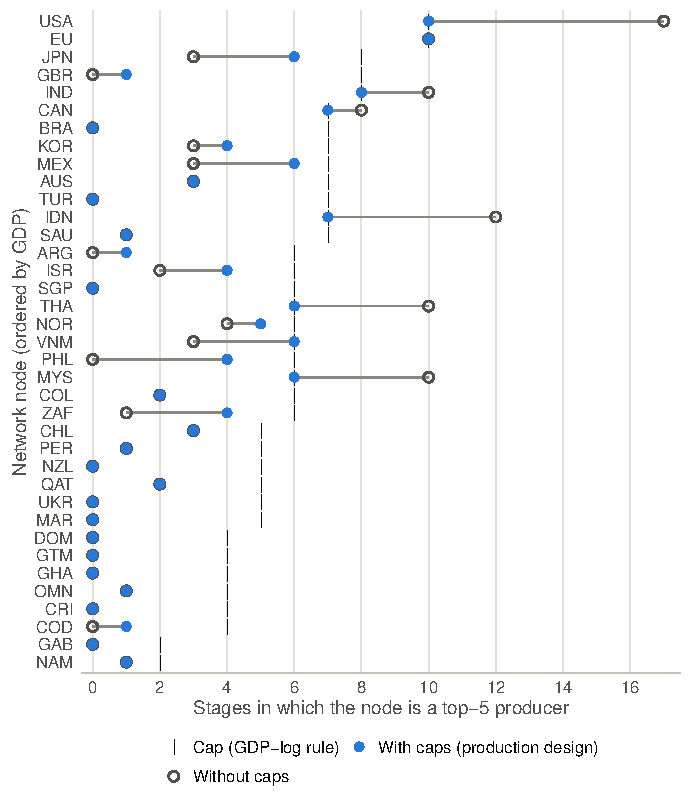
\includegraphics[width=0.75\textwidth]{network_portfolio}
  \caption{Portfolio caps and realised top-5 appearances. For each of the 37 nodes (EU = the
  EU-27 node), ordered by GDP, the vertical tick is the cap $\kappa_i$ of \eqref{eq:net_cap}, the
  filled circle the number of stages in which the node is a top-5 producer \eqref{eq:net_topk} in
  the production design, and the open circle the same count in the design solved without caps and
  otherwise unchanged ($\lambda=0.78$). GDP: latest finite WDI value in current US dollars
  \citep{worldbank2026wdi}, summed over the 27 members for the EU. Source:
  \texttt{allied\_network\_portfolio\_caps.csv}, \texttt{allied\_network\_portfolio\_counts.csv}
  and the no-caps run of the calibration study.}
  \label{fig:network_portfolio}
\end{figure}

% ---------------------------------------------------------------------------
\subsection{What the design does and does not show}
\label{subsec:network_limitations}

Against the five analytical layers of the conceptual source \citep{neis2026allied}, the design joins
the capability layer (node scores) to the complementarity layer (directed edges, with alignment and
Chinese-parent exposure) under a minimal robustness layer (share caps, dual sourcing and the
diversification penalty). It takes the severity layer as given, since all 22 stages are designed
alike, and has no bankability layer; in the source's sequence from severity to coordination to
specialization, it is the last step. Within these limits it illustrates, by construction rather than as a finding, the source's point
that an allocation under a diversification constraint need not follow the ranking of current
exporters; it does not show that the combinations are resilient, because
the program models no shocks.

Four further limits apply. The objective is a score: no unit costs, capacities, ramp-up times or
build costs enter. Stages are solved
independently, so cell manufacturing can be placed where none of the upstream supply is, although
shocks propagate along such links \citep{acemoglu2012network,carvalho2021supply}. The network is
closed: it shows how the coalition could divide its own requirement, not the cost of decoupling
\citep{aiyar2023geoeconomic,javorcik2024economic}. And exposure is direct: dyadic edges do not
register a partner's own dependence on non-members, although the economies that gained U.S. market
share from China are themselves integrated into Chinese supply chains
\citep{freund2024us,alfaro2023global}; the Chinese-parent component of friendshore captures one
channel of such common-mode exposure, ownership, but not shared precursors, equipment or logistics.
